The ground laying principles of the Smartsoft Architecture will be pointed out in the following
Sections. A general overview of how components work together with the Sequencer and the Instruction Planner will be discussed.
As well as the placement of the code (which machine runs which part of the software and also how are they connected).

\section{SmartSoft}
Before the architecture of the Robocup project gets discussed, the SmartsSoft approach is explained in a very brief way. Detailed information about SmartSoft can be found at their homepage \url{http://www.servicerobotik-ulm.de/}.
\\
SmartSoft is a model-driven software development approach (MDSD) in the service robotic systems. It has a strict layer architecture, which divides the implementation process in different pieces, like component development, application building and the end user, which combines via predefined communication patterns distributed components to complex scenarios.
The coordination and implementation of the tasks is represented by the coordination layers of SmartSoft, which are displayed in the figure \ref{fig:architecture_smartsoft_layers}.

\begin{figure}[h]
\centering
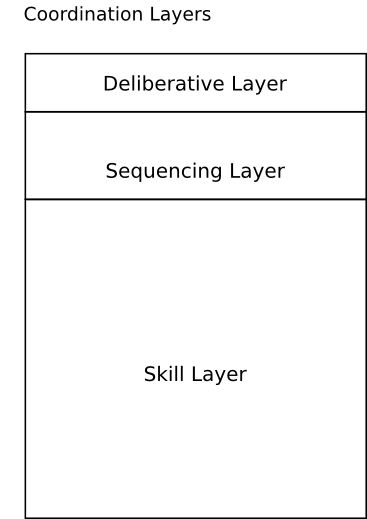
\includegraphics[scale=1.0]{pic/coordination_layers_smartsoft.png}
\caption{Coordination Layers of SmartSoft, http://www.servicerobotik-ulm.de/drupal/?q=node/86}
\label{fig:architecture_smartsoft_layers}
\end{figure}

The general idea is that the components are located in the Skill Layer (e.g. Docking, Detection, LaserScan, ...), because they fulfill a specific task. The Sequencing Layer monitors the situation of the task execution, including coordinating and configuring all other software components in the system. The Deliberative Layer reasons about the high-level goals of the system by using analysis tools, symbolic task planner, constraint solver, etc..

The following figure \ref{fig:architecture_overview} shows the basic architecture of the deployed software on the robots, which are involved at the Robocup. \\

\begin{figure}[h]
\centering
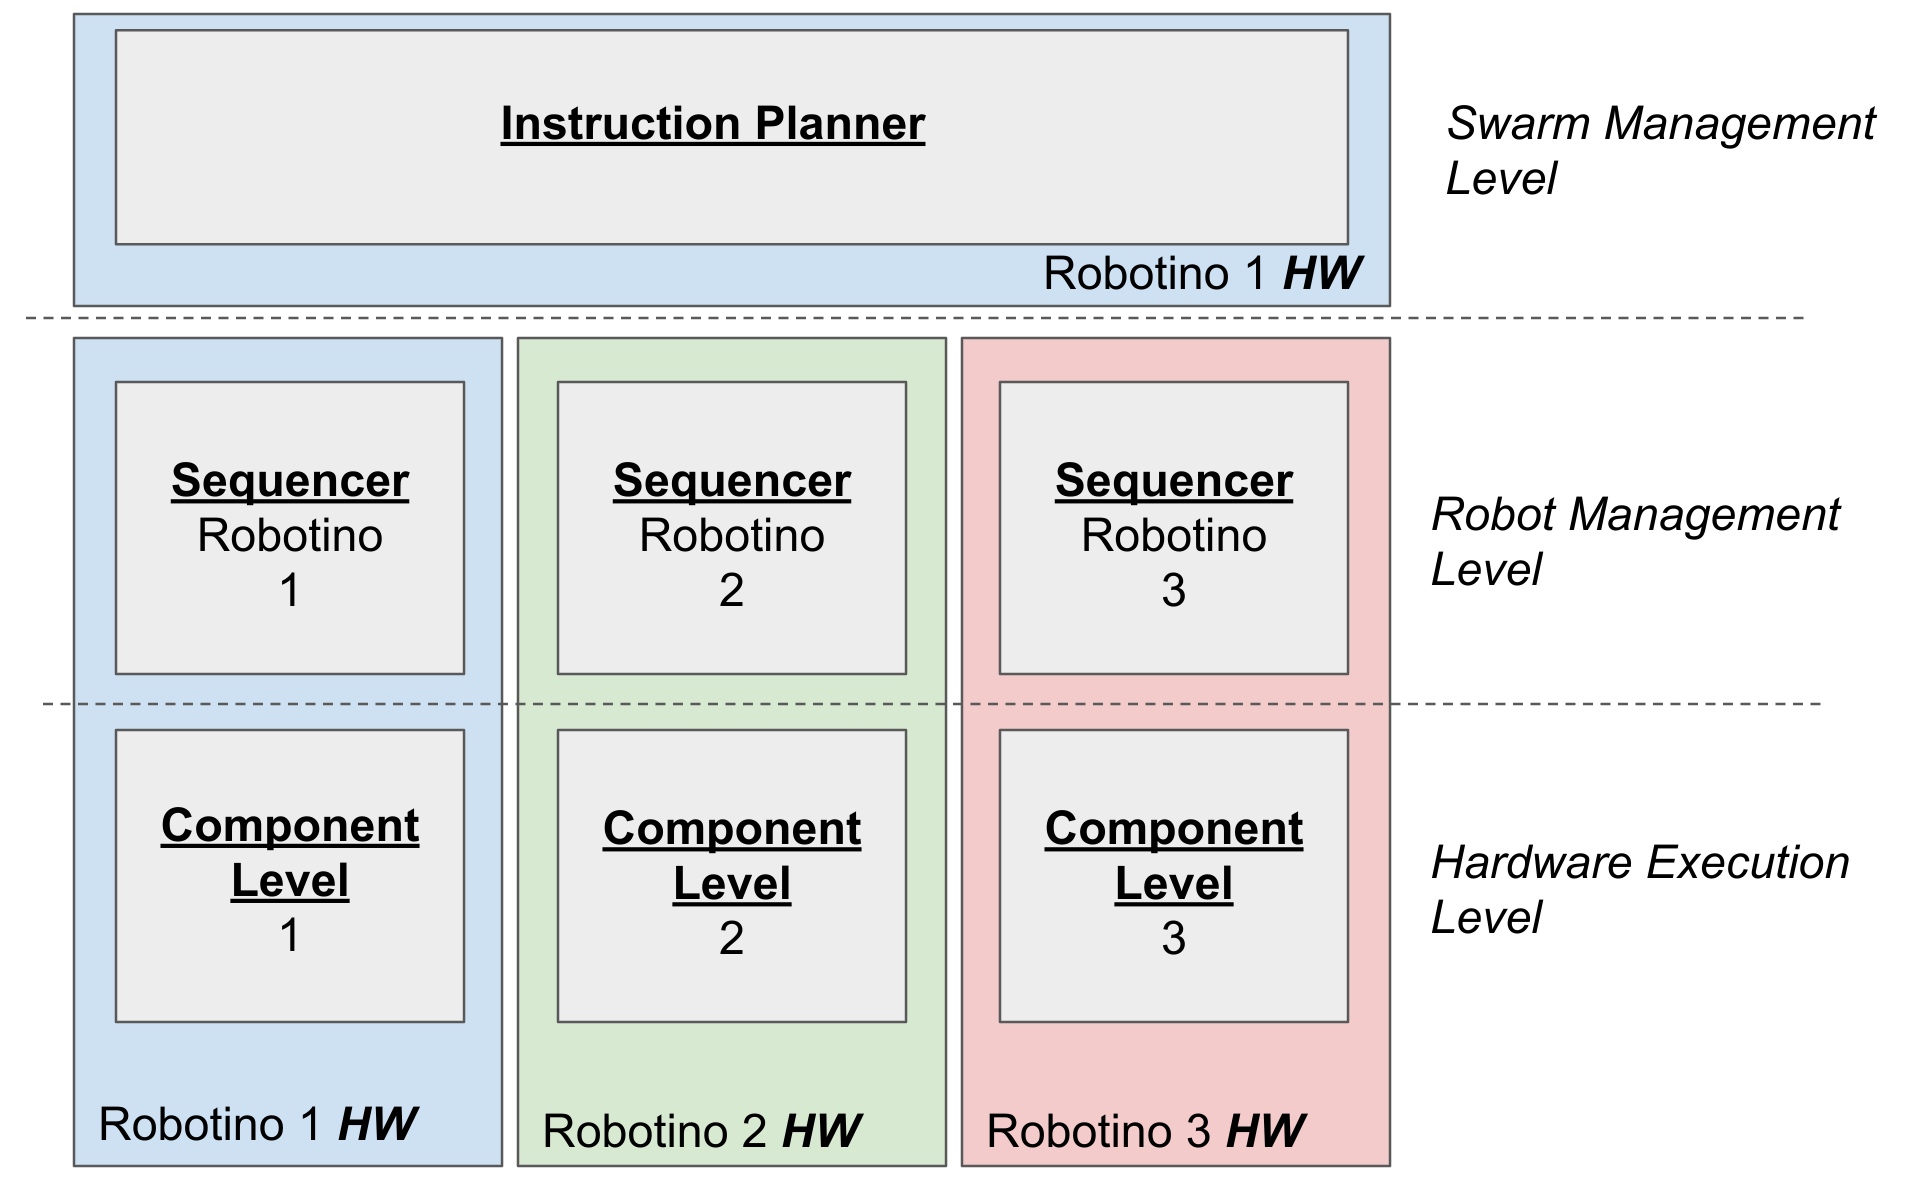
\includegraphics[scale=0.23]{pic/architecture2018.png}
\caption{Arrangement of Components in Architecture}
\label{fig:architecture_overview}
\end{figure}

As seen in the picture above \ref{fig:architecture_overview}, some parts of the system run as a copy on every robot (e.g. the sequencer or movement dependent components), and the Instruction Planner is unique in the complete Robocup scenario. The details of the different components are described in chapter \ref{ch:components}. The following subchapters will give a short description of the involved parts.

\subsection{Instruction Planner}
The Instruction Planner will take care that the task it has been assigned to the system will be handled in a effective way. It consists of multiple parts, the \textbf{Fleet Management} and the \textbf{Objective Management} (see \ref{ch:SmartRobotinoInstructionPlanner}). \\
\\
It actually does not matter on which machine the Instruction Planner is deployed, it could be an external computer, or just one of the robots that are deployed on the field.\\
The limitation is that the instruction planner has to:
\begin{itemize}
    \item have a stable connection to all other robots and to the Refbox
    \item be unique
\end{itemize}
Especially the uniqueness is one point that has to be considered in further progress of the system.
This problem might lead to problems with future deployments of multiple robot systems (see \ref{subsec:Deployments}). \\
\\
The purpose of the Instruction Planner is to keep track of both the game and the robots that are participating.
Based on the information that is provided by all the robots, the Instruction Planner will decide which robot has to perform which task.

\subsection{Sequencer}
The Sequencer is often referred as the \textit{"LispServer"} and manages the events that locally occur on the robot.
Its purpose is to manage all situations that are not "mission critically" and can be solved by the robot itself. \\
A good example is the collision free movement: The robots are able to approach a position on the field without hitting objects in their way. Therefor a coordination of different components is needed, e.g. the \textit{Laser scanner} and the \textit{Moving components}.

These components work together in a way that the received events from the involved components are used to process and delegate further instructions to avoid the crash into objects.
The purpose of the Sequencer is to maintain control of all situations that a single robot can handle on its own, based on the information of events from other components.

\subsection{Components}
Components are the most low level implementations of tasks (e.g. the handling of the movement of the wheels, docking to machines, detection of machines, etc.).
Also all other mentioned parts, as the Sequencer or the Instruction Planner are also components which can be deployed.
All these components communicate with each other using events that are delegated by the Sequencer.
The purpose of the components is the interface to the hardware or software that they handle.
Based on actual sensor values and information delegated by the Sequencer, components fulfill only very fine granular tasks.

\subsection{Deployments}
\label{subsec:Deployments}
Deployments are the connection of all needed components.
A Deployment mostly consists of a map (model driven - code is generated) that describes the connections between all components.
A deployment runs a scenario on a robot (e.g. Robocup - Exploration Phase).

\section{Robocup specific}
The Robocup setup consists of three robots (called Robotinos) and the Referee Box (called Refbox).

\subsection{Robots}
The Robots are the Festo Robotinos, that are equipped with multiple hardware extensions to be able to sense and act
in an industrial (or other indoor) environments.\\
The hardware includes:
\begin{itemize}
    \item \textbf{Camera} - to perform the tag detections
    \item \textbf{Laserscanner} - to sense the environment for objects
    \item \textbf{Gripper} - to be able to move the products around [\textit{needed in Production phase}]
    \item \textbf{5Ghz Wireless LAN} - to communicate with the refbox and other robots
\end{itemize}

The Robotino runs on a Ubuntu 16.04 LTS and can be accessed via VNC / HTTP / SSH.\\

The Robotino is the basis platform that every participant of the RoboCup has to work with.\\
In the contest all Robotinos will be connected to the Refbox and listen for its signals to start the given phases.
The rest of the communication will be performed in a team channel where the Robotinos can exchange messages to each other.
\newpage

\subsection{Referee Box}
The Refbox is the master of the game, and is controlled by a human referee. It takes care of the game progress, as well as the awarding of points and the disqualification of robots.
The Refbox also works event based, so it is bursting out events of the game state (e.g. start / stop or game phases) and receives the messages of the robots to score their points\ref{fig:struct_wRefBox}.
It is also always in contact with all of the robots to ensure that they obey the rules.

\begin{figure}[h]
\centering
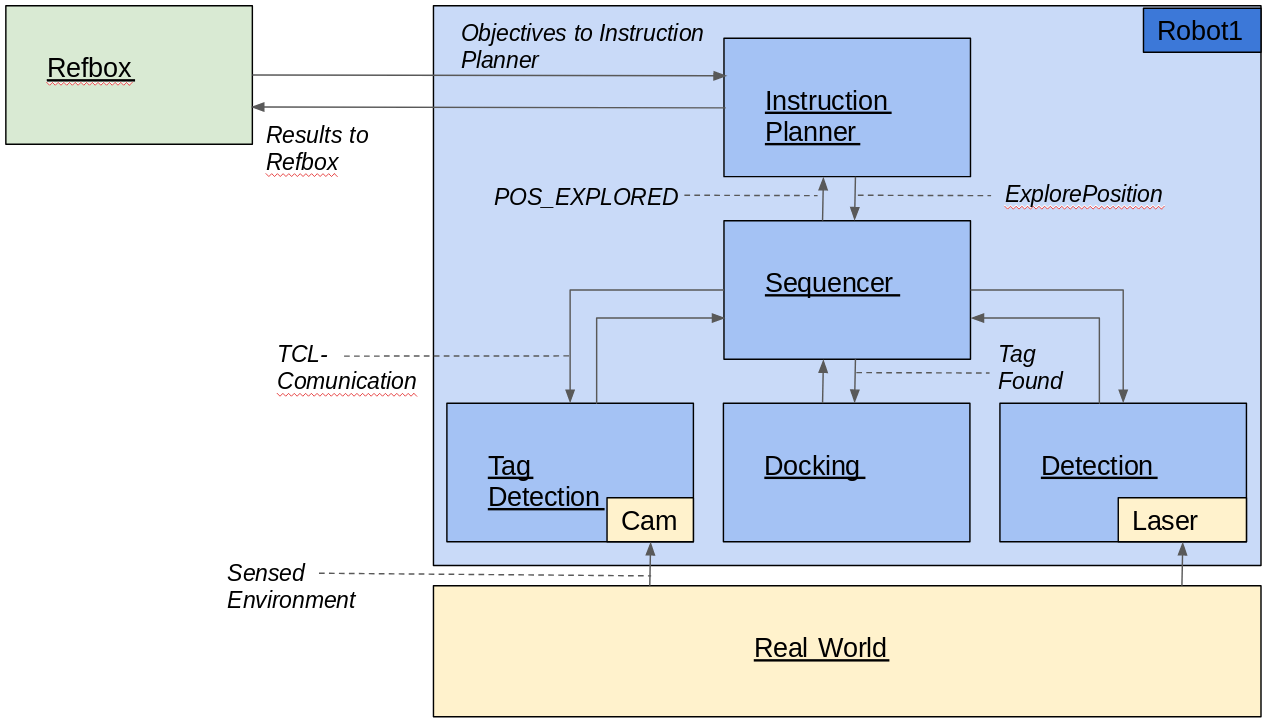
\includegraphics[scale=0.23]{pic/struckture_wRefbo.png}
\caption{Complete System setup of the actually used Robotino}
\label{fig:struct_wRefBox}
\end{figure}
